\usetikzlibrary{positioning, decorations.text}

دایره مورد نظر را به $n$ بخش با مساحت‌های مساوی تقسیم می‌کنیم.
مساحت هر بخش برابر با 
$ \pi (1^2)/n = \pi / n $
خواهد بود.
برای دایره مرکزی خواهیم داشت
\begin{equation}
	\pi r^2 = \pi / n \rightarrow r = \sqrt{1/n}
\end{equation}

و شعاع دایره ناحیه دوم برابر خواهد بود با
\begin{equation}
	\pi R^2 - \pi r^2 = \pi R^2 - \pi / n = \pi / n \rightarrow R = \sqrt{2/n}
\end{equation}

و برای هر ناحیه شماره $i$ داریم
$(r = r_{i-1}, R = r_i)$
\begin{equation}
	\pi R^2 - \pi r^2 = \pi / n \rightarrow R = \sqrt{\frac{1}{n} + r^2}
\end{equation}

تعریف:
$$r_i = \text{شعاع دایره i ام}$$

ادعا:
شعاع دایره محیطی ناحیه $i$ 
برابر است با 
$\sqrt{\frac{i}{n}}$

اثبات با استقرا:

برای پایه استقرا٫ صحت فرض را به ازای $i =2$ در بالا نشان دادیم٫
و فرض را برای 
$i-1$
دایره اول درست فرض می‌کنیم.

اثبات برای $i$
\begin{equation}
	R = \sqrt{\frac{1}{n} + r^2} = \sqrt{\frac{1}{n} + (\sqrt{\frac{i-1}{n}})^2}
	= \sqrt{\frac{1}{n}+\frac{i-1}{n}} = \sqrt{\frac{i}{n}}
\end{equation}

\begin{figure}
\centering
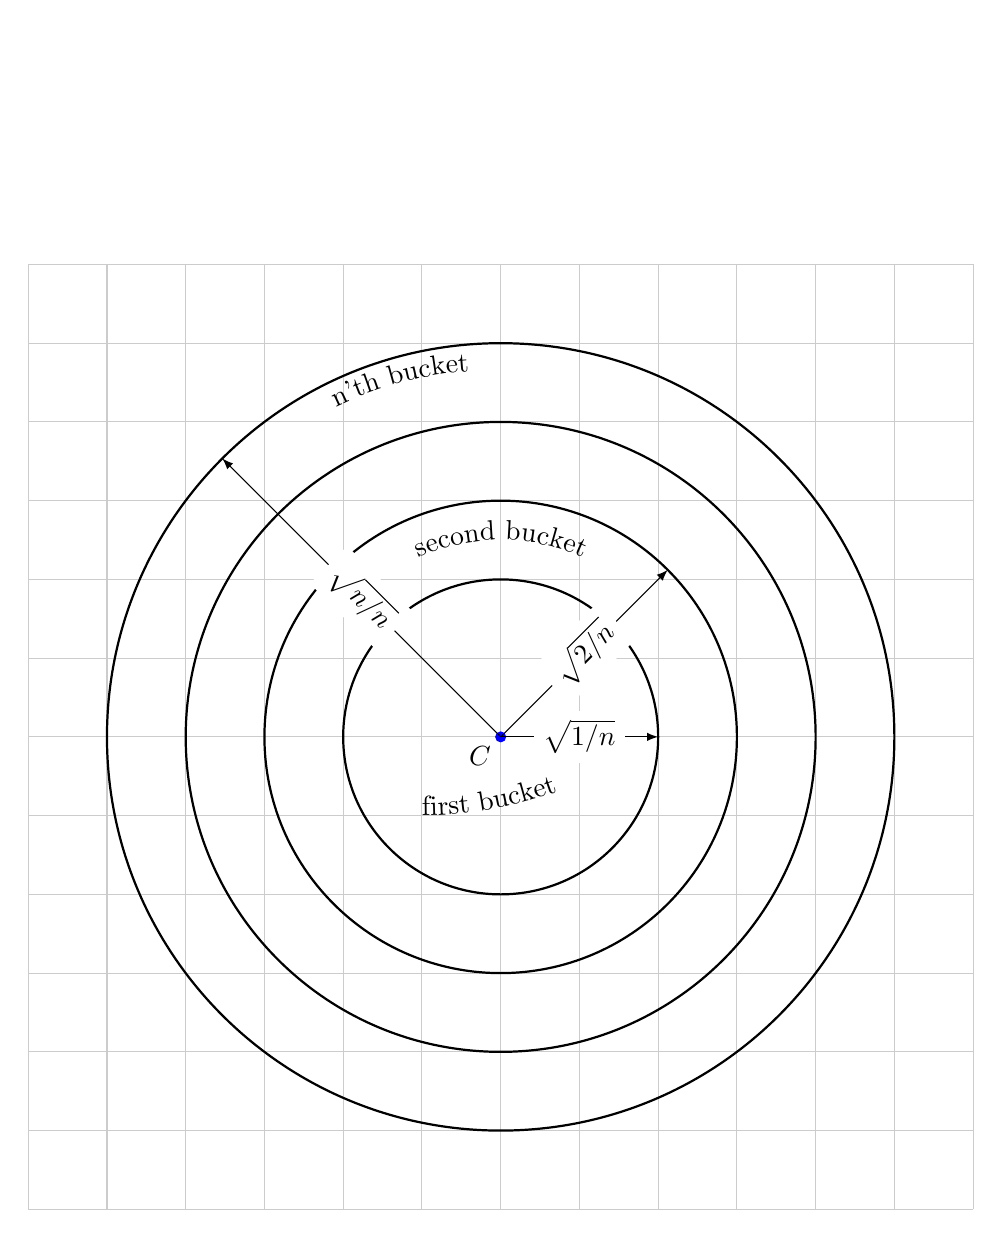
\begin{tikzpicture}[scale=1.0]
\draw [step=1.0,thin,gray!40] (-3,-6) grid (9,6);
\fill[blue] (3,0) circle (2pt) node [black,below left] {$C$};
\draw[thick] (3,0) circle(3);
\draw[thick] (3,0) circle(4);
\draw[thick] (3,0) circle(5);
\draw[thick] (3,0) circle(2);
\begin{scope}[>=latex]
\draw[->] (3,0) -- (5,0)  node [midway,fill=white] {$\sqrt{1/n}$};
\draw[->] (3,0) -- ++(45:3)  node [midway,sloped,fill=white] {$\sqrt{2/n}$};
\draw[->] (3,0) -- ++(-225:5)  node [midway,sloped,fill=white] {$\sqrt{n/n}$};
\end{scope}

\draw [decorate, decoration={text along path, text = second bucket, text align = center}] (0.5,0) arc (180:0:2.5 cm); 

\draw [decorate, decoration={text along path, text = n'th bucket, text align = center}] (-1,2.4) arc (150:60:4.5 cm); 

\draw [decorate, decoration={text along path, text = first bucket}] (2,-1) arc (-90:90:5); 
\end{tikzpicture}
\caption{دایره را به $n$ ناحیه با مساحت مساوی تقسیم کردیم}
\end{figure}

حال مسئله اصلی را حل می‌کنیم.

با توجه به فرض سوال٫ از آن‌جایی که متوسط تعداد نقاط در هر ناحیه متناسب با مساحت آن ناحیه است
اگر دایره را به ناحیه‌های هم مساحت تقسیم کنیم به طور میانگین در هر ناحیه یک نقطه خواهیم داشت.

اگر از الگوریتم
\lr{bucket sort}
استفاده کنیم:
\begin{equation}
	T(n) = \Theta(n) + \sum_{i=1}^n (n_i) ^ 2
\end{equation}

که 
$n_i$
تعداد نقاط در ناحیه 
$i$
است.

و اگر امید ریاضی مرتبه‌ زمانی را حساب کنیم
\begin{equation}
	E[T(n)] = E[\Theta(n) + \sum_{i=1}^n (n_i) ^ 2]
\end{equation}

بعد دو مرحله استفاده از خاصیت خطی‌بودن امیدریاضی
\begin{equation}
	E[T(n)] = E[\Theta(n)] + \sum_{i=1}^n E[n_i ^ 2]
\end{equation}

اگر تعریف کنیم
\begin{equation}
	X_{ij} = \begin{cases}
		1 & \mbox{
		point i being in area j
		} \\
		0 & \mbox{otherwise} 
	\end{cases}
\end{equation}

خواهیم داشت
\begin{equation}
	n_j = \sum_{i=0} ^n X_{ij} 
\end{equation}

پس
\begin{equation}
	E[n^2_i] = E[(\sum_{j=0} ^n X_{ji})^2] = E[\sum_{j=0} ^n X_{ji}^2] + E[\sum_{j=0} ^n \sum_{k=0} ^n 2 X_{ji} X_{ki}]
\end{equation}

برای بخش اول از آن‌جایی که احتمال وجود نقطه در هر ناحیط برابر و برابر با 
$\frac{1}{n}$
است داریم
\begin{equation}
	E[X^2_{ji}] = (1-\frac{1}{n}) * 0^2 + \frac{1}{n} * 1^2 = \frac{1}{n}
\end{equation}
\begin{equation}
	E[\sum_{j=0} ^n X_{ji}^2] = \sum_{j=0} ^n E[X_{ji}^2] = n \cdot \frac{1}{n} = 1
\end{equation}

و برای بخش دوم با توجه با استقلال
$X_{ji}$
و
$X_{ki}$
داریم
\begin{equation}
	E[\sum_{j=0} ^n \sum_{k=0} ^n 2 X_{ji} X_{ki}] = \sum_{j=0} ^n \sum_{k=0} ^n 2 E[X_{ji}] E[X_{ki}] = {n \choose 2} \cdot 2\cdot\frac{1}{n}\cdot \frac{1}{n} = \frac{n(n-1)}{n^2} = 1 - \frac{1}{n}
\end{equation}

و در نتیجه 
\begin{equation}
	E[n_i ^ 2] = 2 - \frac{1}{n}
\end{equation}

در نهایت خواهیم داشت
\begin{equation}
	E[T(n)] = E[\Theta(n)] + \sum_{i=1}^n 2 - \frac{1}{n} = 
	\Theta(n) + 2n - n(1/n) = \Theta(n) + O(n)
\end{equation}






